% 坐标平移示意：P(x,y) → P'(x+a, y+b)
\documentclass[tikz,border=4pt]{standalone}
\usepackage{ctex}
\usepackage{amsmath}
\usetikzlibrary{arrows.meta}
\begin{document}
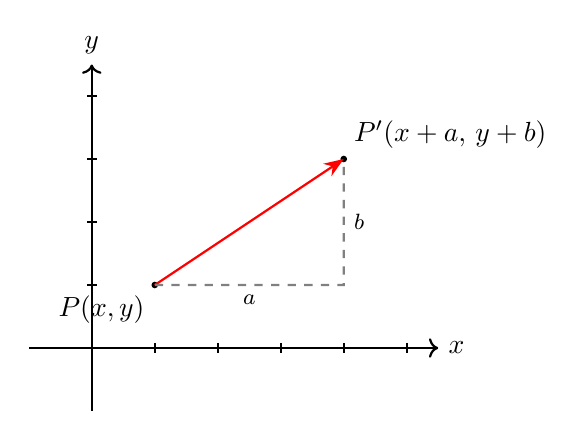
\begin{tikzpicture}[scale=0.8, thick]
  \draw[->] (-1,0) -- (5.5,0) node[right]{$x$};
  \draw[->] (0,-1) -- (0,4.5) node[above]{$y$};
  \foreach \i in {1,2,3,4,5} \draw (\i,0.08) -- (\i,-0.08);
  \foreach \i in {1,2,3,4} \draw (0.08,\i) -- (-0.08,\i);

  \coordinate (P) at (1,1);
  \coordinate (Pp) at (4,3);
  \fill (P) circle (1.5pt);
  \fill (Pp) circle (1.5pt);
  \draw[red, -{Stealth[length=2.5mm]}, thick] (P) -- (Pp);
  \node[below left]  at (P)  {$P(x,y)$};
  \node[above right] at (Pp) {$P'(x+a,\, y+b)$};

  % a 段水平虚线
  \draw[gray, dashed] (P) -- (4,1) -- (Pp);
  \node[below] at (2.5,1) {\footnotesize $a$};
  \node[right] at (4,2)   {\footnotesize $b$};
\end{tikzpicture}
\end{document}
